Una onda electromagnética incidente sobre una superficie en un ángulo arbitrario puede analizarse descomponiendo el problema en dos casos canónicos de polarización\footnote{La polarización es la dirección del campo eléctrico. En nuestro análisis, se considera polarización lineal, de modo que el campo eléctrico en distintos puntos del espacio siempre puede ser representado por vectores colineales.}: perpendicular (TE, transversal eléctrico) o paralela (TM, transversal magnético) al plano de incidencia, que es el formado por el rayo incidente y la normal a la interfaz. El problema de la incidencia perpendicular a la interfaz combina ambos casos.

\begin{figure} [H]
	\centering 
	\subfigure[Polarización paralela (TM).]{
		\label{fig:oblique_incidence_parallel}
		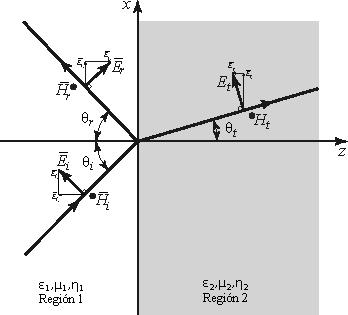
\includegraphics[width=0.45\textwidth]{intro_electro/incidencia_oblicua_paralela-version2.pdf}}
	\hspace{5mm}
	\subfigure[Polarización perpendicular (TE).]{
		\label{fig:oblique_incidence_perp}
		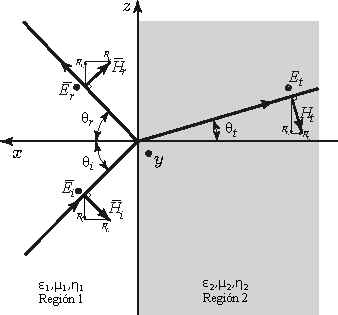
\includegraphics[width=0.45\textwidth]{intro_electro/incidencia_oblicua_perpendicular-version2.pdf}}
	\caption{Incidencia oblicua para los dos casos de polarización analizados.}
	\label{fig:oblique_incidence}
\end{figure}

Los campos eléctrico y magnético incidentes, según el sistema de coordenadas definido en la Figura \ref{fig:oblique_incidence}, pueden ser expresados, en forma general, usando las expresiones \ref{eq:electric_field_wave_solution} y \ref{eq:relacion-e-h-ondaplana}, y considerando que no hay pérdidas, como indican las ecuaciones \ref{eq:incident_fields}:

\begin{align}
	\label{eq:incident_fields}
	\vec{E}_i &= \vec{E}_0 \;e^{-j\vec{\beta}_1 \cdot \vec{r}} &
	\vec{H}_i = \frac{\hat{\beta}_1 \times \vec{E}_0}{\eta_1} \;e^{-j\vec{\beta}_1 \cdot \vec{r}}
\end{align}

donde $\vec{r}=(x,y,z)$, $\vec{\beta}_1 = \hat{\beta}_1 \;\omega \sqrt{\mu_1 \epsilon_1}$. $\hat{\beta}_1$ es la dirección de propagación de la onda plana, y $\eta_1 = \sqrt{\mu_1 / \epsilon_1} = j\omega \mu / \gamma$ es la impedancia de onda de región de incidencia.

Se define al coeficiente de reflexión $\Gamma$ como la relación entre la magnitud del campo reflejado y del campo incidente, $E_r / E_i$. De la misma manera, el coeficiente de transmisión $T$ es la relación entre el módulo del campo transmitido al segundo medio y el campo incidente desde el primer medio, $E_t / E_i$, de manera que $1+\Gamma = T$ y que $(1-\Gamma)/\eta_1 = T/\eta_2$. 

Usando estos coeficientes, a partir de las ecuaciones \ref{eq:incident_fields}, y teniendo en cuenta las condiciones de borde descriptas en la Sección \ref{sec:condiciones-borde}, se pueden calcular los campos reflejados y transmitidos. Para los dos casos canónicos analizados, los campos incidentes, reflejados y transmitidos se resumen en la tabla \ref{table:incidencia_oblicua}, así como los coeficientes de reflexión y transmisión.

\tabulinesep=1.2mm
\taburulecolor{black!20}
\begin{table}
	
	\begin{tabu} to 1\textwidth {gX[c]@{}X[c]@{}}
		\rowcolor{black!20} & \multicolumn{1}{c}{\textbf{TM}} & \multicolumn{1}{c}{\textbf{TE}}\\
		$\vec{E}_i$
		&
		\scalebox{0.86}{%
			$
			E_0\; (\hat{z}\; \mathrm{cos}\; \theta_i + \hat{x}\; \mathrm{sin}\; \theta_i)\; e^{-j \beta_1 (z\; \mathrm{sin}\; \theta_i - x\; \mathrm{cos}\; \theta_i)}
			$
		}	
		&
		\scalebox{0.86}{%
			$
			E_0\; \hat{y} \;e^{-j \beta_1 (z\; \mathrm{sin}\; \theta_i - x\; \mathrm{cos}\; \theta_i)}
			$
		} \\
		$\vec{H}_i$
		&
		\scalebox{0.86}{%
			$
			\frac{E_0}{\eta_1}\; \hat{y}\; e^{-j \beta_1 (z\; \mathrm{sin}\; \theta_i - x\; \mathrm{cos}\; \theta_i)}
			$
		}
		&
		\scalebox{0.86}{%
			$
			\frac{E_0}{\eta_1} \;(-\hat{z}\; \mathrm{cos}\; \theta_i - \hat{x}\; \mathrm{sin}\; \theta_i)\; e^{-j \beta_1 (z\; \mathrm{sin}\; \theta_i - x\; \mathrm{cos}\; \theta_i)}
			$
		} \\
		\hline
	
		$\vec{E}_r$
		&
		\scalebox{0.86}{%
			$
			E_0\; \Gamma\; (\hat{z}\; \mathrm{cos}\; \theta_r - \hat{x}\; \mathrm{cos}\; \theta_r)\; e^{-j \beta_1 (x\; \mathrm{sin}\; \theta_r + z\; \mathrm{sin}\; \theta_r)}
			$
		}	
		&
		\scalebox{0.86}{%
			$
			E_0\; \Gamma\; \hat{y} \;e^{-j \beta_1 (z\; \mathrm{sin}\; \theta_r + x\; \mathrm{cos}\; \theta_r)}
			$
		} \\
		$\vec{H}_r$
		&
		\scalebox{0.86}{%
			$
			-\frac{E_0\; \Gamma}{\eta_1}\; \hat{y}\; e^{-j \beta_1 (x\; \mathrm{sin}\; \theta_r + z\; \mathrm{sin}\; \theta_r)}
			$
		}
		&
		\scalebox{0.86}{%
			$
	 		\frac{E_0\; \Gamma}{\eta_1} \;(\hat{z}\; \mathrm{cos}\; \theta_r - \hat{x}\; \mathrm{sin}\; \theta_r)\; e^{-j \beta_1 (z\; \mathrm{sin}\; \theta_r + x\; \mathrm{cos}\; \theta_r)}
			$
		} \\
	\hline
		$\vec{E}_t$
		&
		\scalebox{0.86}{%
			$
			E_0\; T\; (\hat{z}\; \mathrm{cos}\; \theta_t + \hat{x}\; \mathrm{sin}\; \theta_t) e^{-j \beta_2 (z\; \mathrm{sin}\; \theta_t - x\; \mathrm{cos}\; \theta_t)}
			$
		}
		&
		\scalebox{0.86}{%
			$
			E_0\; T\; \hat{y}\; e^{-j \beta_2 (z\; \mathrm{sin}\; \theta_t - x\; \mathrm{cos}\; \theta_t)}
			$
		} \\
		$\vec{H}_t$
		&
		\scalebox{0.86}{%
			$
	 		\frac{E_0\; T}{\eta_1}\; \hat{y}\; e^{-j \beta_2 (z\; \mathrm{sin}\; \theta_t - x\; \mathrm{cos}\; \theta_t)}
			$
		}
		&
		\scalebox{0.86}{%
			$
			\frac{E_0\; T}{\eta_2}\; (-\hat{z}\; \mathrm{cos}\; \theta_t - \hat{x}\; \mathrm{sin}\; \theta_t)\; e^{-j \beta_2 (z\; \mathrm{sin}\; \theta_t - x\; \mathrm{cos}\; \theta_t)}
			$
		} \\
		\hline
		
		$\Gamma$
		&
		$\frac{\eta_2\; \cos\; \theta_t - \eta_1 \; \cos\; \theta_i}{\eta_2\; \cos\; \theta_t + \eta_1 \; \cos\; \theta_i}$
		&
		$\frac{\eta_2\; \cos\; \theta_i - \eta_1 \; \cos\; \theta_t}{\eta_2\; \cos\; \theta_i + \eta_1 \; \cos\; \theta_t}$
		\\
		$T$
		&
		$\frac{2 \;\eta_2 \; \cos\; \theta_i}{\eta_2\; \cos\; \theta_t + \eta_1 \; \cos\; \theta_i}$
		&
		$\frac{2\; \eta_2 \; \cos\; \theta_i}{\eta_2\; \cos\; \theta_i + \eta_1 \; \cos\; \theta_t}$
	\end{tabu}
	\caption{Campos incidentes, transmitidos y reflejados, y coeficientes de reflexión y transmisión para incidencia oblicua de una onda plana sobre una interfaz dieléctrica.}
	\label{table:incidencia_oblicua}
\end{table}

Si se fuerza la continuidad de las componentes tangenciales de los campos sobre la interfaz para ambos casos, $\vec{E}_i^{tg} + \vec{E}_r^{tg} = \vec{E}_t^{tg}$ y $\vec{H}_i^{tg} + \vec{H}_r^{tg} = \vec{H}_t^{tg}$, se obtienen las expresiones \ref{eq:continuidad_campos_paralelo} para el modo TM, y \ref{eq:continuidad_campos_perpendicular} para el modo TE.

\begin{equation}
	\begin{aligned}
		cos \; \theta_i \; e^{-j \beta_1 z \sin \; \theta_i} + \Gamma \; cos \; \theta_r \; e^{-j \beta_1 z \; \sin\; \theta_r} &= T\; \cos\; \theta_t \; e^{-j \beta_2 z \; \sin\; \theta_t}\\
		\frac{1}{\eta_1} \; e^{-j \beta_1 z \; \sin \theta_i} - \frac{\Gamma}{\eta_1} \; e^{-j \beta_1 z \; \sin \; \theta_r} &= \frac{T}{\eta_2} \; e^{-j \beta_2 z \; \sin\; \theta_t}
	\end{aligned}
	\label{eq:continuidad_campos_paralelo}
\end{equation}

\begin{equation}
	\begin{aligned}
		e^{-j \beta_1 z \sin \; \theta_i} + \Gamma \; e^{-j \beta_1 z \; \sin\; \theta_r} &= T\; e^{-j \beta_2 z \; \sin\; \theta_t}\\
		-\frac{1}{\eta_1} \cos\; \theta_i \; e^{-j \beta_1 z \; \sin \theta_i} - \frac{\Gamma}{\eta_1} \; \cos\; \theta_r e^{-j \beta_1 z \; \sin \; \theta_r} &= -\frac{T}{\eta_2} \; \cos\; \theta_t \; e^{-j \beta_2 z \; \sin\; \theta_t}
	\end{aligned}
	\label{eq:continuidad_campos_perpendicular}
\end{equation}

En estas ecuaciones se observa que a ambos lados de las igualdades, las expresiones son funciones de la posición sobre la interfaz. Para que la condición de borde se cumpla en todos sus puntos, la variación en $z$ debe ser la misma en todos los términos, de forma que el efecto de la variación sea anulado: $\beta_1 \; \sin\; \theta_i = \beta_1 \; \sin \; \theta_r = \beta_2 \; \sin\; \theta_t$.  De esta consideración se deriva la Ley de Snell (asumiendo que $\mu_1 = \mu_2$), expresada en la ecuación \ref{eq:snell_law}. En la gráfica de la Figura \ref{fig:ley_snell} se puede observar el comportamiento del ángulo de refracción según en ángulo de incidencia, sobre una interfaz entre aire y FR4, en sentidos opuestos.

\begin{subequations}
	\label{eq:snell_law}
	\begin{align}
	\theta_i &= \theta_r\\
	\beta_1 \; \sin\; \theta_i = \beta_2 \; \sin\; \theta_t & \overset{\eta=\omega\mu/\beta}{\Longrightarrow} \eta_2 \; \sin\; \theta_i = \eta_1 \; \sin\; \theta_t  \label{eq:snell_law_second}
	\end{align}
\end{subequations}

\begin{figure}[htp]
	\centering
	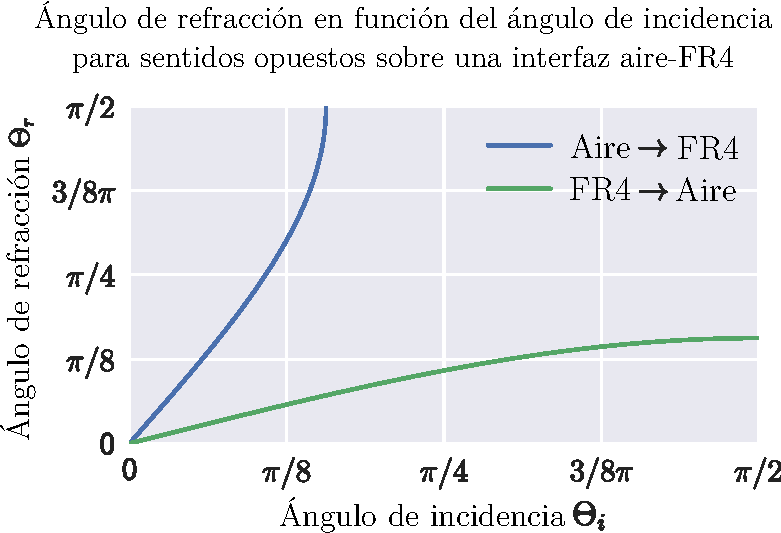
\includegraphics[width=0.7\textwidth]{intro_electro/angulo-refraccion-snell.pdf}
	\caption{Ángulo de refracción en función del ángulo de incidencia, según la ley de Snell.}
	\label{fig:ley_snell}
\end{figure}

Utilizando estas expresiones, y a partir de las ecuaciones \ref{eq:continuidad_campos_paralelo} y \ref{eq:continuidad_campos_perpendicular}, se obtienen las expresiones para los coeficientes de reflexión y transmisión de la tabla \ref{table:incidencia_oblicua}. Resulta importante destacar que, para el caso de incidencia perpendicular ($\theta_i = 0$), los coeficientes quedan simplificados a $\Gamma = (\eta_2 - \eta_1)/(\eta_2 + \eta_1)$ y $T = (2 \; \eta_2)/(\eta_2 + \eta_1)$.

Los coeficientes de transmisión y reflexión para incidencia oblicua, en ambas polarizaciones, se pueden graficar en función del ángulo incidente, teniendo en cuenta las ecuaciones de Snell para expresar el ángulo de transmisión en función del ángulo de incidencia. Estas gráficas se muestran, para la interfaz aire-FR4, en la Figura \ref{fig:coeficientes-aire-fr4}, donde, además,  teniendo en cuenta la constante de propagación compleja de la ecuación \ref{eq:constante-propagacion-compleja}, se graficó también el caso con pérdidas, donde se observa, en general, una mayor reflexión y, por tanto, menor transmisión. Para ángulos de incidencia rasantes, la transmisión es mínima y la reflexión es máxima.

Resulta ilustrativo, además, graficar el comportamiento según el ángulo de incidencia de la misma interfaz, pero en el sentido dieléctrico-aire. Este gráfico se observa en la Figura \ref{fig:coeficientes-fr4-aire}, donde los coeficientes de transmisión pueden ser mayores a 1 porque el ángulo en el segundo medio es menor al de incidencia, permitiendo conservar el flujo de energía por unidad de área.

\begin{figure}[H]
	\centering 
	\subfigure[Coeficiente de reflexión entre aire y FR4 en función de $\theta_i$.]{
		\label{fig:coeficiente-reflexion-aire-fr4}
		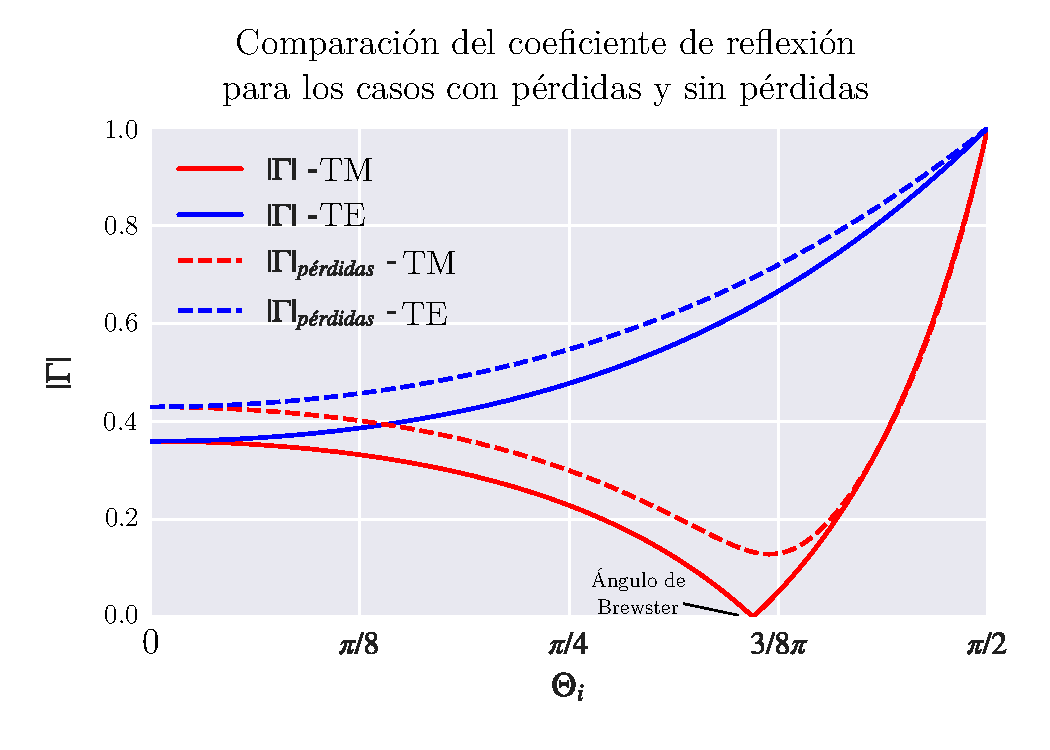
\includegraphics[width=0.48\textwidth]{intro_electro/plot-comparacion-lossy-lossless-annotated.pdf}}
	\subfigure[Coeficiente de transmisión entre aire y FR4 en función de $\theta_i$.]{
		\label{fig:coeficiente-transmision-aire-fr4}
		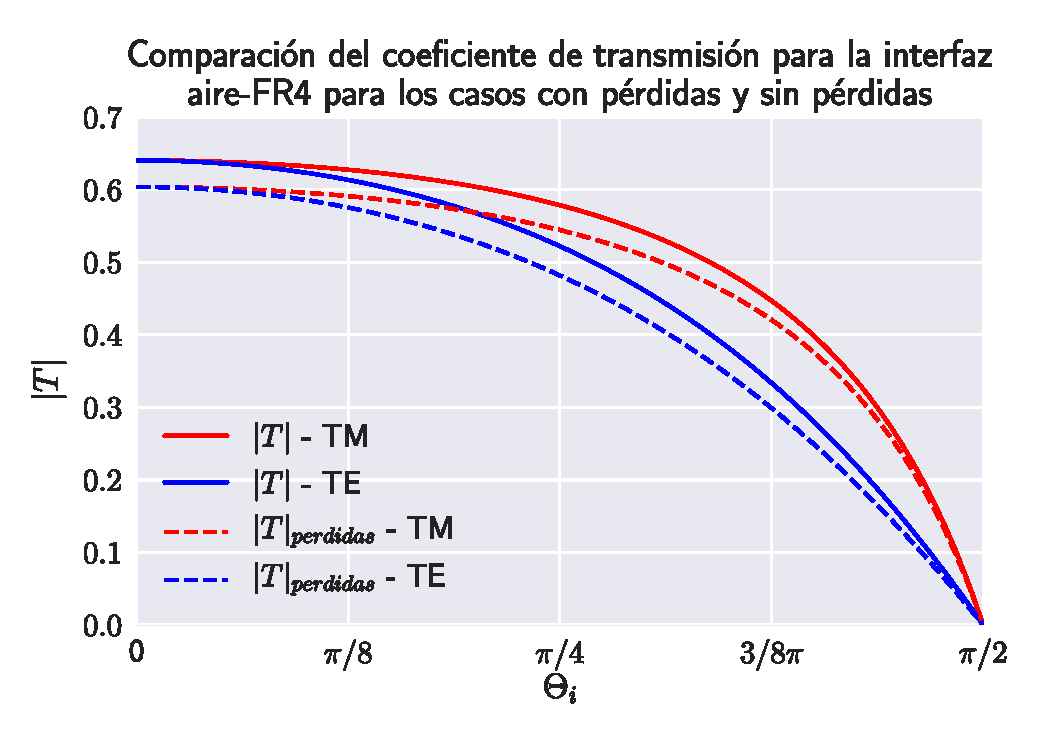
\includegraphics[width=0.48\textwidth]{intro_electro/plot-comparacion-lossy-lossless-T.pdf}}
	\caption{Coeficientes de transmisión y reflexión para el caso en que el medio de incidencia es aire, y el medio de transmisión es FR4.}
	\label{fig:coeficientes-aire-fr4}
\end{figure}


\begin{figure}[htp]
	\centering
	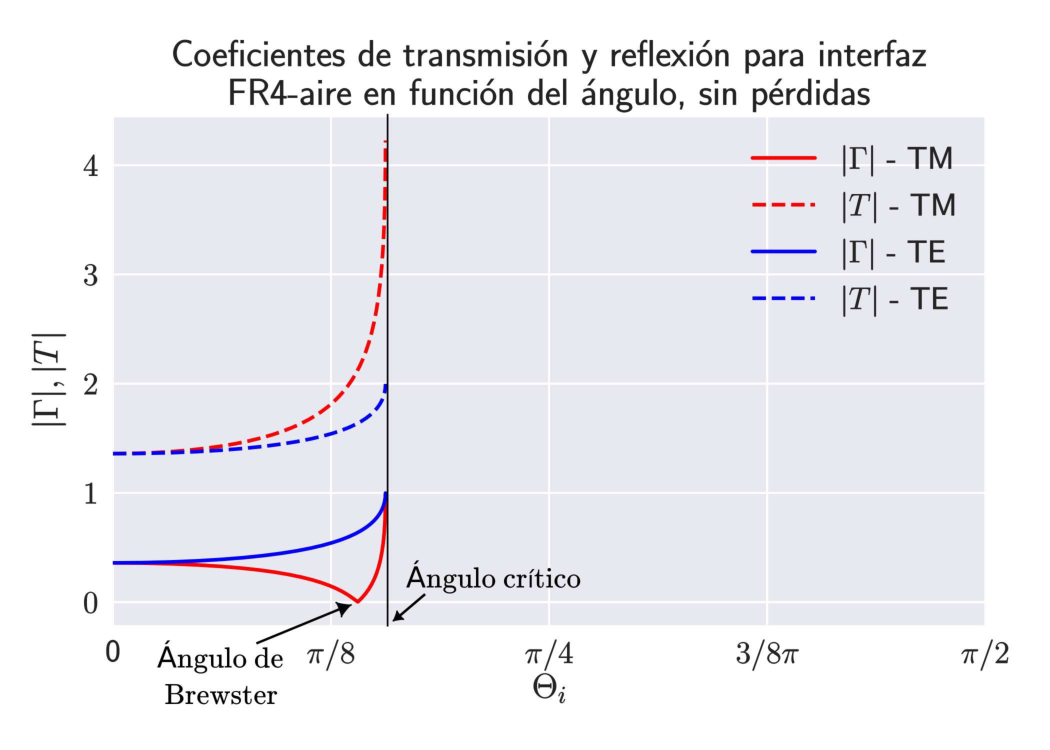
\includegraphics[width=0.7\textwidth]{intro_electro/plot-coeficientes-fresnel-dirInversa.pdf}
	\caption{Comportamiento de los coeficientes de reflexión y transmisión para el caso de incidencia FR4-aire.}
	\label{fig:coeficientes-fr4-aire}
\end{figure}



\section{Ángulo de Brewster y ángulo crítico}

Se conoce como ángulo de Brewster al ángulo de incidencia $\theta_i$ necesario para que se produzca reflexión nula ($\Gamma = 0$) en una interfaz, cuando sobre ella incide una onda plana en forma oblicua. Este efecto se da únicamente para la polarización TM, es decir, cuando existe componente de campo eléctrico en la dirección normal a la interfaz, por lo que suele ser utilizado como mecanismo para lograr polarización de una onda electromagnética.

Si se anulan los coeficientes de reflexión mostrados en la tabla \ref{table:incidencia_oblicua}, y se utilizan las ecuaciones \ref{eq:snell_law}, se puede deducir que la polarización TE no presenta ángulo de Brewster\footnote{Para lograr reflexión nula en TE se requiere que $\sin \; \theta_i / \sin \; \theta_t = cos \; \theta_i / cos \; \theta_t = \eta_1 / \eta_2$, lo cual es imposible.}, aunque sí lo hace la polarización TM\footnote{Para lograr reflexión nula en TM se requiere que $\sin \; \theta_i / \sin \; \theta_t = cos \; \theta_t / cos \; \theta_i = \eta_1 / \eta_2$, lo cual no supone una contradicción. Multiplicando la ecuación \ref{eq:snell_law_second} y el valor de $\Gamma$ para polarización TM, se obtiene que $\sin\;\theta_i \; cos \; \theta_i = \sin \; \theta_t \; cos \; \theta_t$, ó $\sin \; 2\theta_i = \sin \; 2\theta_t$, que se satisface cuando $2\theta_i = \pi - 2\theta_t$, de modo que $\theta_i + \theta_t = \pi/2$.}, cuando $\theta_i + \theta_t = \pi/2$. Aplicando esta condición en la Ley de Snell (ecuación \ref{eq:snell_law_second}) se obtiene la expresión del ángulo de Brewster:

%%% GRAFICAR LO DE ACA ARRIBA, REEMPLAZANDO THETA_T POR LA LEY DE SNELL. EJE X: THETA_I. DE ESTA MANERA SE PODRIA VERIFICAR QUE PARA TE NO HAY SOLUCION Y PARA TM SI.

\begin{align}
	\label{eq:Brewster_angle}
	\tan\;\theta_B &= \frac{\eta_1}{\eta_2} = \sqrt{\frac{\epsilon_2}{\epsilon_1}}
\end{align}

Como se observa en la Figura \ref{fig:Brewster-funcion-epsilon}, el ángulo de Brewster tiende a $90^{\circ}$ cuando la permeabilidad eléctrica del segundo medio es mucho mayor a la del primero, lo que significa que para evitar reflexiones, el ángulo de incidencia debe ser rasante. Cuando se da el caso contrario, en que la permeabilidad eléctrica del medio incidente es mayor a la del medio de transmisión, el ángulo de Brewster se vuelve menor a $45^{\circ}$, de lo que se deduce que una incidencia \textit{casi} perpendicular a la interfaz, y en consecuencia con polarización \textit{cercana} a TEM (aunque no exactamente TEM) lograría evitar la reflexión. El ángulo de $45^{\circ}$ cuando las permeabilidades eléctricas de ambos medios son iguales es meramente anecdótico, ya que si no existen diferencias entre los dos medios que forman la interfaz, la misma no existe, y por lo tanto no hay onda reflejada para \textit{ningún} ángulo de incidencia.

\begin{figure} [H]
	\centering 
	\subfigure[Ángulo de Brewster en función de $\epsilon_2/\epsilon_1$.]{
		\label{fig:Brewster-funcion-epsilon}
		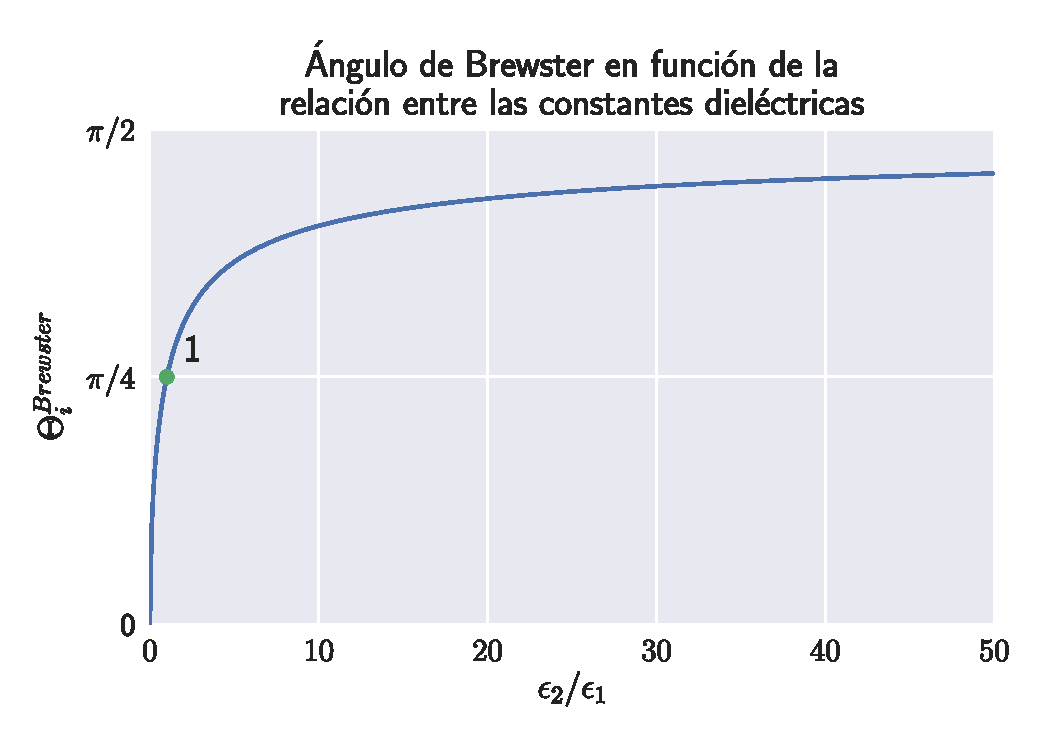
\includegraphics[width=0.48\textwidth]{intro_electro/plot-brewster.pdf}}
	\subfigure[Ángulo crítico y rango de reflexión total en función de $\epsilon_2/\epsilon_1$.]{
		\label{fig:angulo-critico-funcion-epsilon}
		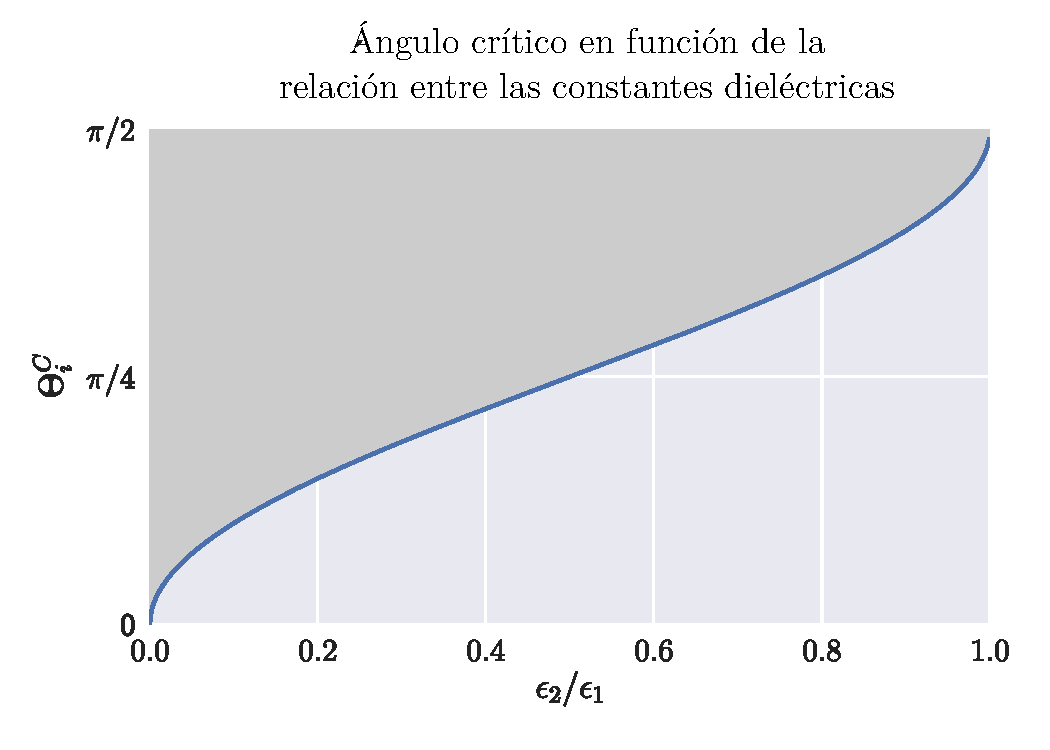
\includegraphics[width=0.48\textwidth]{intro_electro/plot-angulo-critico.pdf}}
	\caption{}
	\label{fig:angulo-critico-epsilon}
\end{figure}

En la figura  \ref{fig:coeficientes-aire-fr4} se puede observar el comportamiento de los coeficientes de reflexión y transmisión alrededor del ángulo de Brewster para polarización TM, cuando no se consideran pérdidas. Para polarización TE, el ángulo de Brewster no existe, y una situación similar se da cuando existen pérdidas en los materiales, incluso para polarización TM. En la Figura \ref{fig:coeficientes-fr4-aire} también se puede observar el fenómeno de ángulo de Brewster, aunque debido a la dirección de la onda incidente, el mismo es mucho menor.


En ángulo crítico se define como el ángulo de incidencia para el cual la onda incidente es totalmente reflejada, y la onda transmitida no se propaga a la segunda región.

Si se observan las expresiones del coeficiente de transmisión de la tabla \ref{table:incidencia_oblicua}, el único valor de $\theta_i$ para el cual la transmisión es nula es $\pi/2$, es decir, incidencia rasante. Sin embargo, a partir de la ecuación \ref{eq:snell_law_second}, se obtiene que $\sin \; \theta_t = \eta_2 / \eta_1\; \sin\; \theta_i$. Se puede observar que en los casos en que $\eta_2 > \eta_1$ es posible que el ángulo de transmisión alcance el valor $\pi/2$ antes de que lo haga en ángulo de incidencia. El ángulo crítico, entonces, surge de la expresión \ref{eq:angulo_critico}, graficada en la Figura \ref{fig:angulo-critico-epsilon}. En la gráfica se puede observar que si $\epsilon_2 = \epsilon_1$, el único ángulo para el que hay reflexión completa es el rasante. A medida que disminuye la relación entre las permeabilidades dieléctricas, el valor del ángulo crítico disminuye, hasta que el valor de la permitividad dieléctrica del segundo medio es mucho mayor a la del primero, lo que vuelve a las impedancias de onda muy disimiles, generando que haya reflexión total para cualquier ángulo de incidencia.

\begin{equation}
	\label{eq:angulo_critico}
	\sin\; \theta_i^c = \frac{\eta_1}{\eta_2}\;\sin \; \theta_t|_{\theta_t=\pi/2} = \sqrt{\frac{\epsilon_2}{\epsilon_1}} \implies \theta_c = \arcsin \;\sqrt{\frac{\epsilon_2}{\epsilon_1}} = \arcsin \;\frac{\eta_1}{\eta_2}
\end{equation}

Para ángulos mayores a $\theta_c$, las expresiones del coeficiente de reflexión se vuelven complejas y de módulo 1, por lo que toda la energía electromagnética es reflejada, y la onda transmitida tiene un comportamiento evanescente, como se muestra en la Figura \ref{fig:angulo_critico}. En la ecuación \ref{eq:angulo_critico} se observa que si $\theta_i > \theta_c$, el ángulo $\theta_t$ pierde significado físico, debido a que $\sin\; \theta_t$ debería ser mayor a 1 para cumplir la ecuación.

\begin{figure}[htp]
	\centering
	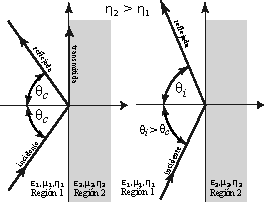
\includegraphics[width=0.6\textwidth]{intro_electro/angulo_critico.pdf}
	\caption{Ilustración del comportamiento de una onda plana durante la incidencia con ángulo critico y con ángulo mayor al $\theta_c$.}
	\label{fig:angulo_critico}
\end{figure}

Se debe notar que en el argumento anterior no se consideró la polarización de la onda incidente, por lo que la reflexión completa se puede dar tanto en modo TM como en modo TE, siempre y cuando la incidencia se produzca desde el medio ópticamente más denso al menos denso \cite{Fernandez:Electromag}, como se muestra en la Figura \ref{fig:coeficientes-fr4-aire}. Sin embargo, resulta útil expresar el comportamiento de los campos.

Para el caso de una onda incidente con una polarización lineal arbitraria como la expresada en la ecuación \ref{eq:incident_fields}, se debe considerar que la componente longitudinal a la interfaz del vector de onda $\vec{\gamma}$ se mantendrá constante, de modo que $\gamma_{2_z} = \gamma_{1_z} = \gamma_1 \; \sin \; \theta_i$. La componente transversal a la interfaz, en cambio, será $\gamma_{2_x} = \gamma_2\; \cos \; \theta_t = \gamma_2 \sqrt{1-sin^2\theta_t} = \gamma_{2_x}$. Dado que para el caso en que el ángulo incidente es mayor al ángulo crítico se requiere que $\sin\;\theta_t > 1$, el valor de ${\gamma_2}_x$ será imaginario, $-i\alpha$ \footnote{El signo negativo se desprende de la imposibilidad física de un crecimiento exponencial del valor del campo, lo cual descarga la posibilidad de que el signo sea positivo}. De esta forma, para direcciones de campos arbitrarias, y teniendo en cuenta el hecho de que el vector $\vec{\gamma}$ se desarrolla sobre el plano de incidencia:

\begin{subequations}
	\begin{align}
		\vec{E}_t (\vec{r},t) = \vec{E}_2 \; e^{-j \vec{\gamma}_2 \cdot \vec{r}} = \vec{E}_2 \; e^{-j({\gamma_2}_x x + {\gamma_2}_z z)} = \vec{E}_2 \; e^{-j(\beta z - j\alpha x)} = \vec{E}_2 \; e^{-j\beta z} \; e^{- \alpha x}\\
		\vec{H}_t (\vec{r},t) = \vec{H}_2 \; e^{-j \vec{\gamma}_2 \cdot \vec{r}} = \vec{H}_2 \; e^{-j({\gamma_2}_x x + {\gamma_2}_z z)} = \vec{H}_2 \; e^{-j(\beta z - j\alpha x)} = \vec{H}_2 \; e^{-j\beta z} \; e^{- \alpha x}
	\end{align}
\end{subequations}

Se observa que en la dirección perpendicular a la interfaz hay un comportamiento evanescente o exponencial decreciente de la onda transmitida, mientras que existe propagación en la dirección paralela a la interfaz, dando lugar a lo que se conoce como onda de superficie.

La ecuación del módulo del vector de onda (\ref{eq:numero_de_onda}) resulta redefinida como $\beta_x^2 - \alpha_z^2 = \gamma_2^2$, de donde se deduce que $\alpha_z = \sqrt{\gamma_x^2\;sin^2\;\theta_i - \gamma_2^2}$.